% !TeX root = Bericht_main.tex
\subsection{Aufgabe 30}
In Aufgabe 30 betrachten wir nochmals die Konvektions-Diffusions-Reaktions-Gleichung 
\begin{align*}
	\partial_t c = \dive ( \kappa_c \nabla c - cq) + r(c) 
\end{align*}
Im Vergleich zur letzten Aufgabe wollen wir nun aber den Reaktionsterm $r(c)$ ändern und so statt exponentiellem Wachstum, logistisches Wachstum betrachten. Während wir also zuvor noch $r(c) = Rc$ für ein $R \in \R$ gesetzt hatten, setzen wir nun $r(c) = r_0 c - r_1 c^2$ für $r_0,r_1 > 0$
\newline
Dazu sind wir wie folgt vorgegangen:
 

 \begin{figure}[H]
 		\centering
 			\captionabove{Implementierung der Klasse HybridReactionProblem\_logistic in Problem.C}
 		\subfigure[Reaction = 2.5]{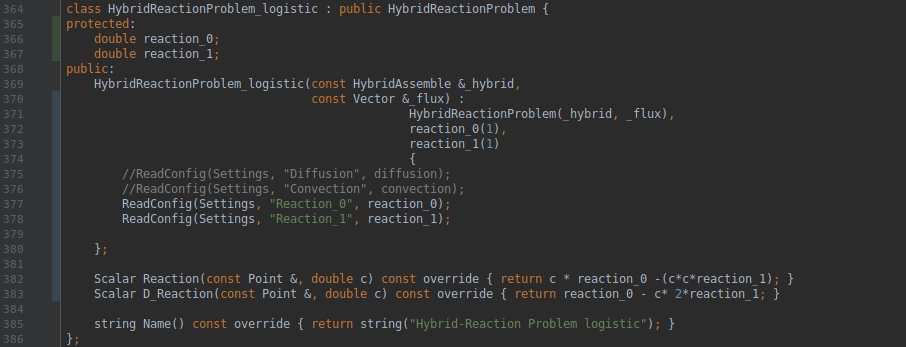
\includegraphics[width=0.99\textwidth]{../Aufgabe30/code.png}}
 \end{figure}

Wir konnten anhand der Massewerte verifizieren, dass für $r_1 = 0 $  gerade wieder, wie zu erwarten ist, das exponentielle Wachstum vorliegt:
\begin{figure}[H]
	\centering
	\captionabove{Verlauf der Masse und des Ausflusses (Konvektion = 0.1)}
	\subfigure[Exponentielles Wachstum Reaction = 2.5]{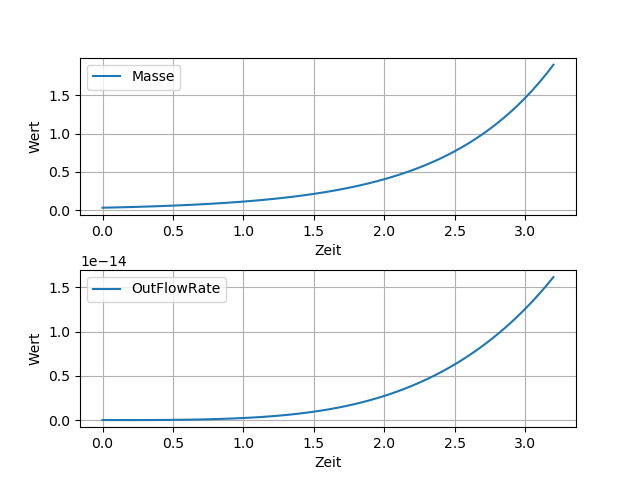
\includegraphics[width=0.49\textwidth]{../Aufgabe27/lowconvecreaction=2.5/plot.png}}
	\subfigure[Logistisches Wachstum $r_0 = 2.5$ $r_1 = 0$  ]{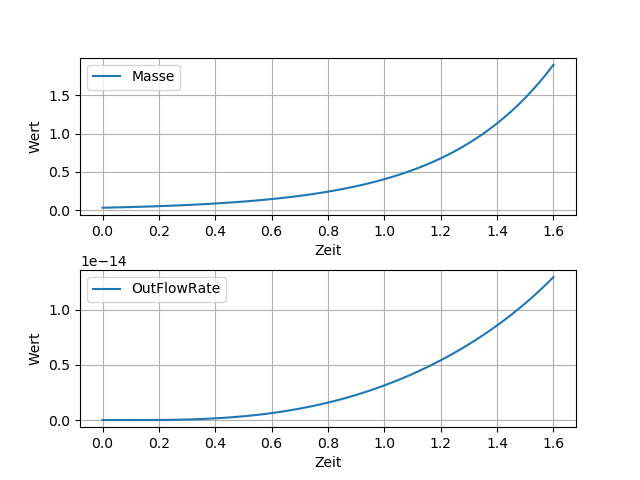
\includegraphics[width=0.49\textwidth]{../Aufgabe30/Vgl30r10/plot.png}}
\end{figure}
Auch der Wert der Masse zum Zeitpunkt $t=1.6$ ist bei beiden Lösungen identisch.
Zugleich konnten wir aber auch das unterschiedliche Verhalten der Masse bezogen auf die Zeit für unterschiedliche $r_1$ nachweisen. 
\begin{figure}[H]
	\label{vergleichsplot}
	\centering
	\captionabove{Vergleich der Masseverläufe für $r_0 = 2.5$ und unterschiedliche $r_1$}
    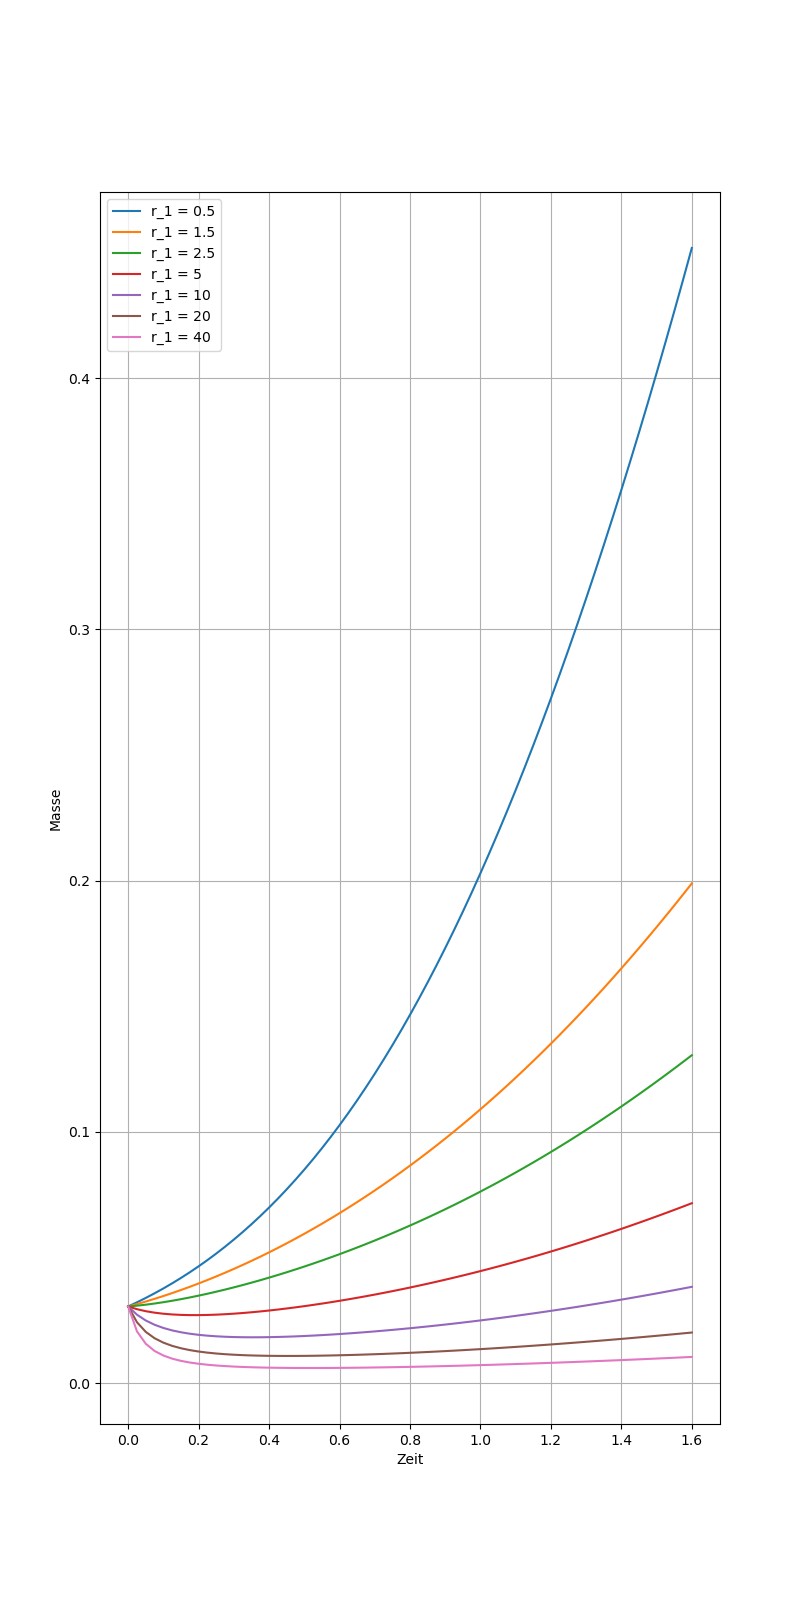
\includegraphics[width=0.80\textwidth]{../Aufgabe30/vergleichsplot.png}
\end{figure}
Man sieht sehr gut, dass sich das Verhalten immer mehr von dem des exponentiellen Wachstums entfernt, je größer wir den Parameter $r_1$ wählen.  
Betrachten wir die Gleichung des logistischen Wachstums genauer, können wir dieses Verhalten auch erklären:
\begin{align*}
	r(c) &= r_0 c - r_1 c^2 \\
	&=r_1c(\frac{r_0}{r_1}-c)
\end{align*}
Für den Grenzwert erhalten wir somit gerade $G = \frac{r_0}{r_1}$
Ist $G >> c_0 $ so erhalten wir auf dem betrachteten Zeitintervall $t \in [0,1.6]$ einen nahezu exponentiellen Verlauf, wie beispielsweise in  Abbildung 6 bei $r_1 = 0.5$. Genauso sieht man für $G<0$ (beispielsweise in Abbildung 6 bei $r_1 = 40$), dass sich der Masseverlauf 'umkehrt' und wir zunächst Masse verlieren, bevor wir uns dem Niveau $G$ annähern.
Für Werte $G \approx c_0 $ bzw. $G$ leicht größer als $c_0$ erwarten wir eigentlich einen 'typisch logistischen' Verlauf, dieser ist aber sehr schwer zu erreichen, da die vorliegenden Größen von Diffusion und Ausfluss (welcher von der Konvektion abhängt) durch fortwährende kleine Masseverluste ein solches Verhalten nahezu verhindern.
\newline
In der folgenden Abbildung wird aber vielleicht zumindest dieser 'typisch logistische' Verlauf deutlich, auch wenn das Abflachen des Masseplots nicht allein durch die Annäherung an den Grenzwert, sondern auch durch den (wenn auch schwach) ansteigenden Ausfluss zu erklären ist. 
\begin{figure}[H]
	\centering
	\captionabove{Masse und Ausflussverhalten bei $r_0 = 10 $ und $r_1 = 4.9 $}
	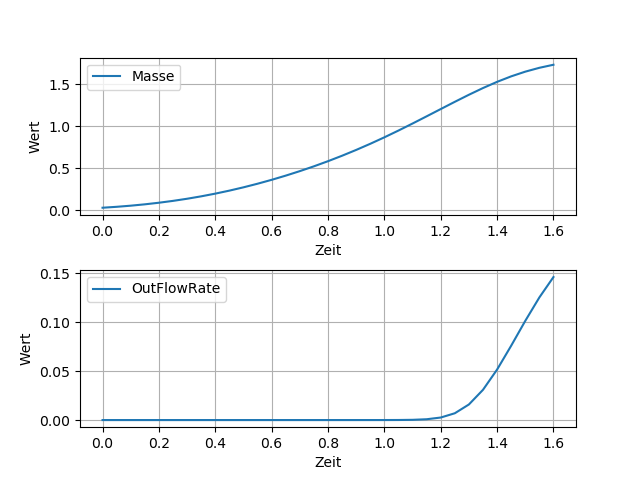
\includegraphics[width=0.80\textwidth]{../Aufgabe30/Testvltgut/plot.png}
\end{figure}

Außerdem erwähnenswert ist, dass es möglich ist bei bestimmten Werten für $r_0$ und $r_1$ in dem verwendeten Verfahren das in der Vorlesung vorgestellte Implizite Euler-Verfahren mit Newton-Iteration in jedem Zeitschritt wiederzuerkennen.
Nachfolgender Auschnitt zeigt einen Schritt für $r_0 = 40$ , $r_1=19.9$ , $dt = 0.05$ , $dt_{min}=0.0125$:
\begin{figure}[H]
	\centering
	\captionabove{Newton-Iteration für den ersten Eulerschritt}
	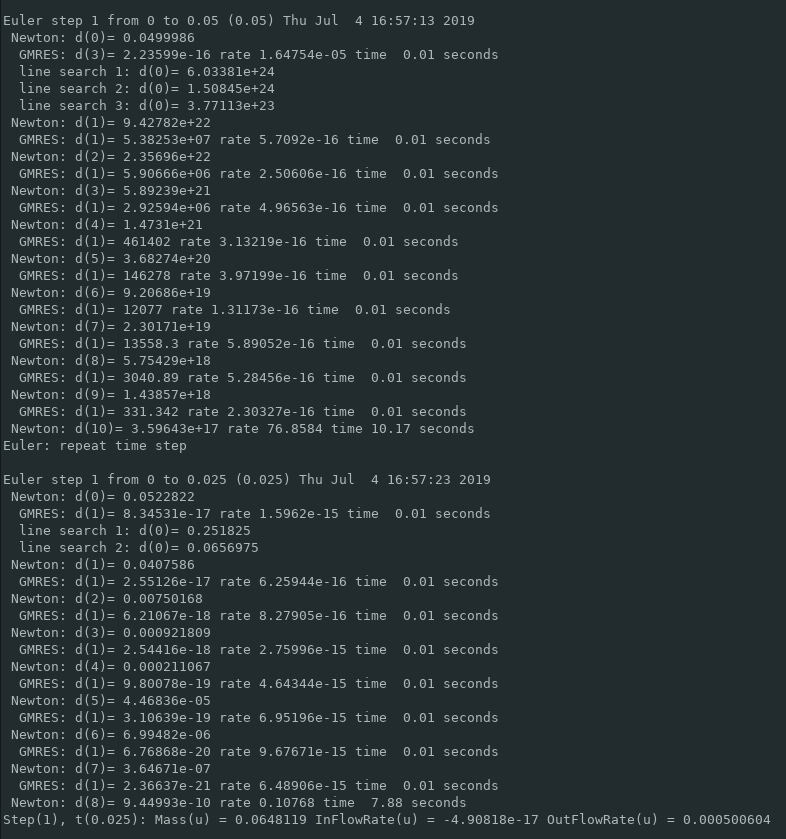
\includegraphics[width=0.80\textwidth]{../Aufgabe30/algorithmus.png}
\end{figure}
Vor allem erkennt man sehr schön zum einen die lineare Suche, welche aufgerufen wird, wenn der Wert der Newton-Iteration zu schlecht ist zum anderen erkennt man auch den Schritt 8) sehr schön: 
Falls nämlich keine Konvergenz vorliegt, wird im Verfahren der Eulerschritt mit der halben Zeitschrittweite erneut durchgeführt. Dies geschieht entweder solange, bis $dt_{min}$ erreicht wurde, oder (wie in obigem Fall) ein zufriedenstellendes Ergebnis vorliegt.
